\section{计算机硬件}


%\begin{frame}\ft{\subsecname}
%\begin{figure}
%\centering
%\animategraphics[height=2.in,autoplay,controls,buttonsize=0em,loop]{12}{ch01/fig/computer_}{0}{3}
%\end{figure}
%\end{frame}

 

\begin{frame}\ft{硬件}
\begin{itemize}
\item 中央处理器(Central Processing Unit, CPU) \\
\item 存储器 \\
\begin{itemize}
	\item 内存(Memory) \\
	\item 外存 
	\begin{AutoMultiColItemize}
		\item 硬盘
		\item 软盘
		\item 光盘
		\item U盘
	\end{AutoMultiColItemize}
\end{itemize}
\item 输入设备 
\begin{AutoMultiColItemize}
	\item 键盘
	\item 鼠标
	\item 摄像头
	\item 扫描仪
\end{AutoMultiColItemize}
\item 输出设备\begin{AutoMultiColItemize}
	\item 显示器
	\item 打印机
	\item 音响
	\item 绘图仪
\end{AutoMultiColItemize}
\end{itemize}
\end{frame}

\begin{frame}[fragile]\ft{主板}
\begin{figure}[h] 
	\centering
	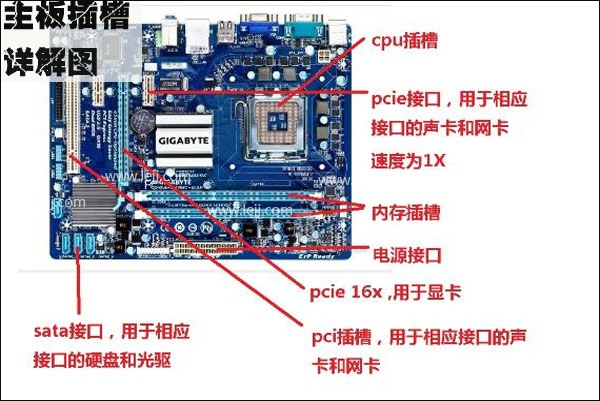
\includegraphics[width=\textwidth]{ch01/fig/mobo}
\end{figure}
\end{frame}


\begin{frame}\ft{主板}
{CPU、内存、硬盘、显卡、声卡等都安装在\red{主板}上。}

\begin{itemize}
\item
将电脑的各个部件连接起来。 \\[0.1in]
\item
提供各种外接设备的接口,如:
\begin{AutoMultiColItemize}
\item USB接口
\item 键盘接口
\item 鼠标接口
\item 网线接口
\end{AutoMultiColItemize}
\end{itemize}
\end{frame}






\begin{frame}[fragile]\ft{CPU}
\begin{figure}[h] 
\begin{minipage}[t]{0.45\linewidth}
\centering
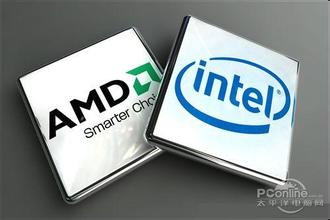
\includegraphics[width=\textwidth]{ch01/fig/cpu1}
\end{minipage}
\hfill
\begin{minipage}[t]{0.45\linewidth}
\centering
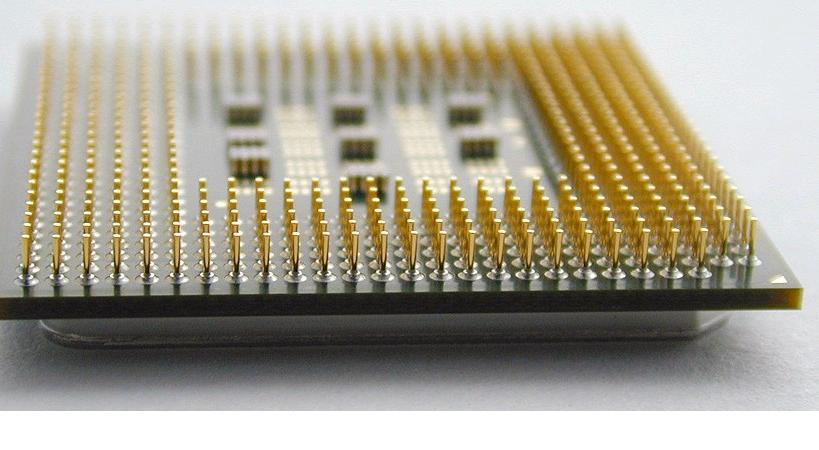
\includegraphics[width=\textwidth]{ch01/fig/cpu2}
\end{minipage}
\end{figure}
\end{frame}

\begin{frame}\ft{CPU}
CPU是计算机的大脑。

\red{计算机处理数据的能力主要取决于CPU。}  \vspace{.1in}

三种基本操作: 

\begin{itemize}
\item \red{读数据}:一般从内存读取数据。 \\[0.1in]
\item \red{处理数据}:通过算术逻辑单元对数据进行处理。 \\[0.1in]
\item \red{写数据}:将数据写入内存。
\end{itemize}

\end{frame}

\begin{frame}\ft{CPU}
 
CPU一般由以下四部分组成:
\begin{itemize}
\item  \red{运算器(算术逻辑单元)} \quad 处理数据 
\begin{itemize}
\item 算术运算:加、减、乘、除 
\item 逻辑运算:与、或、非、异或
\end{itemize} 
\item  \red{控制器}  \quad 对指令译码,并且发出为完成每条指令所要执行的各个操作的控制信号。\\[.1in]
\item  \red{寄存器}  \quad 保存指令执行过程中临时存放的寄存器操作数和中间(或最终)的操作结果。 
\begin{AutoMultiColItemize}
\item 通用寄存器
\item 专用寄存器
\item 控制寄存器
\end{AutoMultiColItemize}

\item \red{高速缓冲存储器} \quad 在CPU芯片内,是一个读写速度比内存更快的存储器。
%当CPU向内存中写入或读出数据时,这个数据也被存储进高速缓冲存储器中。当CPU再次需要这些数据时,CPU就从高速缓冲存储器读取数据,而不是访问较慢的内存,当然,如需要的数据在Cache中没有,CPU会再去读取内存中的数据。
\end{itemize}
\end{frame}
 
\begin{frame}\ft{内存}
\begin{figure}
\centering
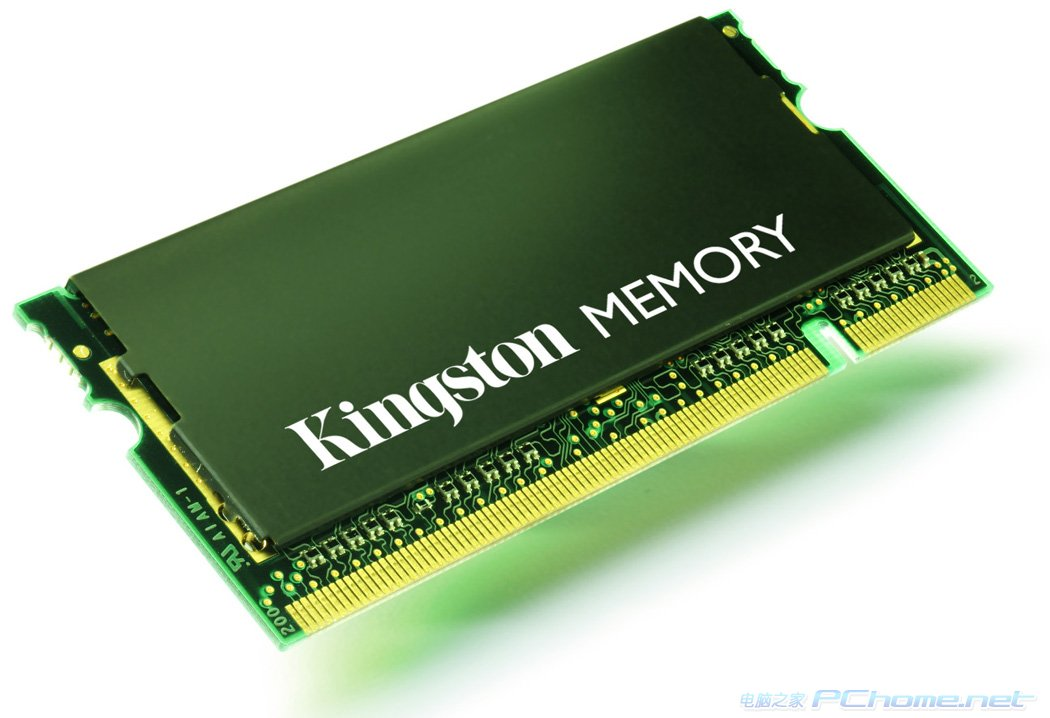
\includegraphics[width=3in]{ch01/fig/memory} 
\end{figure}
\end{frame}
 
\begin{frame}\ft{内存}
\begin{itemize}
\item 内存是CPU能直接寻址的存储空间,所有程序的运行都是在内存中进行的。\\[0.1in]
\item
只要计算机在运行中,CPU就会把需要运算的数据调到内存中进行运算,当运算完成后CPU再将结果传送出来。\\[0.1in]
\item
其作用是用于暂时存放CPU中的运算数据,以及与硬盘等外部存储器交换的数据。\\[0.1in]
\end{itemize}
 \end{frame}
 
 \begin{frame}\ft{内存}
 

\begin{itemize}
\item \red{只读存储器(Read Only Memory, ROM)} 
\item[] 只能读取,不能写入。即使断电,里面的数据也不会丢失,一般用于存放计算机的基本程序和数据。\\[0.1in] 
\item \red{随机存储器(Random Access Memory, RAM)}
\item[] 既可读取,也可写入。断电时,里面的数据就会丢失。{内存条就是将RAM集成块集中在一起的一小块电路板。}\\[0.2in]

\end{itemize}
 \end{frame}
 
\begin{frame}[fragile]\ft{各类存储器的逻辑连接}
\begin{figure}[h] 
\centering
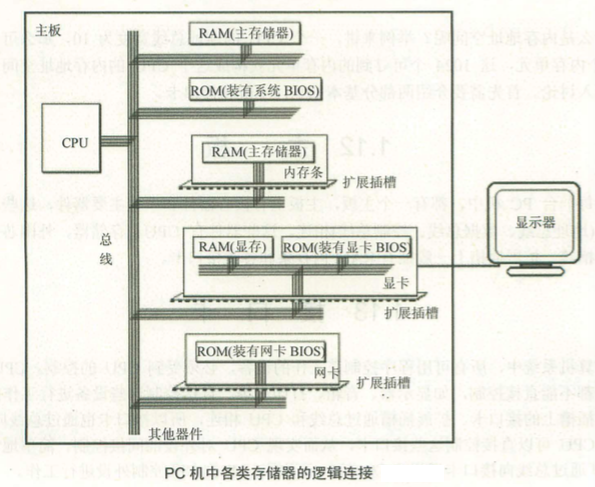
\includegraphics[width=3.7in]{ch01/fig/PCLink}
\end{figure}
\end{frame}
